\documentclass[border=10pt]{standalone}
\usepackage{pgfplots}
\pgfplotsset{compat=1.18}
\begin{document}
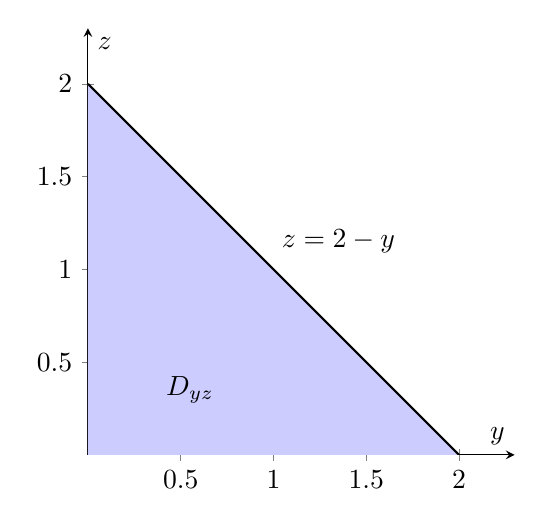
\begin{tikzpicture}
\begin{axis}[
    axis lines=middle,
    xlabel=$y$, ylabel=$z$,
    xmin=0, xmax=2.3, ymin=0, ymax=2.3,
    width=7cm, height=7cm,
    samples=120,
    ]
\addplot[fill=blue!20, draw=none, domain=0:2] {2-x} \closedcycle;
\addplot[domain=0:2, thick, black] {2-x};
\node at (axis cs:1.35,1.15) {$z=2-y$};
\node at (axis cs:0.55,0.35) {$D_{yz}$};
\end{axis}
\end{tikzpicture}
\end{document}